% !TEX root = ../thesis-example-en.tex
\chapter{Experimental setup and tools}\label{sec:setup}
\begin{flushright}
    \begin{minipage}{0.85\textwidth}
        \small
        Part of the work presented in this chapter is employed in: \\
        \preamblecite{zhuObservationPlaidlikeSpin2024}
    \end{minipage}
\end{flushright}
\section{Introduction}

\section{NV microscopy}

At the heart of the SQM system is the NV center, its optical readout and coherent control. To realize this, a confocal microscope paired with microwave (MW) instrumentation is necessary, attached to a cryogenic system. This necessitates additional constraints regarding mounting and size when designing the optical system. Some of the essential components and considerations to make a NV microscopy optical system suitable for use with the AD2200, are explained in detail here.

The AD2200 is equipped with a relatively long ($\sim\qty{1}{\meter}$) sample stick that is inserted in to the center of the cryostat. Due to the requirement of better thermal isolation from ambient conditions, the sample stick (essentially an optical cage system) has its structural rods constructed partially from insulating teflon-like material. This renders very good cryogenic performance but cause difficulty in optical alignment due to its lack of rigidity. The stick is further inserted into  a low clearance tube with the cold gaseous \ce{He} environment. This tube is rigid, and defines then the end configuration of the sample stick. The optics is therefore constructed as a cage system based optical `head' that is permanently mounted to the top of the sample stick.

The optical head is a standalone confocal microscope excitation and collection system requiring only the input of excitation laser with an SM-Fiber and output of collected light via an SM/MM-Fiber. The optical head incorporates the following functions:
\begin{itemize}
    \item Collimation and steering of excitation beam
    \item Steering and focussing of collection beam
    \item Polarization control of excitation beam
    \item Imaging of back reflection from sample
    \item Spectral and spatial filtering for confocal microscopy
\end{itemize}

The use of the cage system allows for permanent mounting of the optics head onto the sample stick due to its integrated design and light weight. The lasing and detection system is built on small mobile optical table that allows with only two fiber connections between the optics head and itself. To enable easier handling, the optics head and sample stick (amounting to $\sim\qty{8}{\kilo\gram}$) are inserted/retracted from the cryostat using a crane built onto the cryostat frame. This also ensures that the relatively low rigidity sample stick is not bent and maintains optical alignment. 

\subsection*{Excitation system}

The excitation system is designed as a standalone unit that can be easily separated from the optical head where it is connected to with one single mode fiber. The system itself is built on a mobile optical table, allowing easy access around the cryostat when necessary. This also allows easy alignment of the optical system independent of the optical head. 

\begin{figure}[h]
    \centering 
    \centering 
    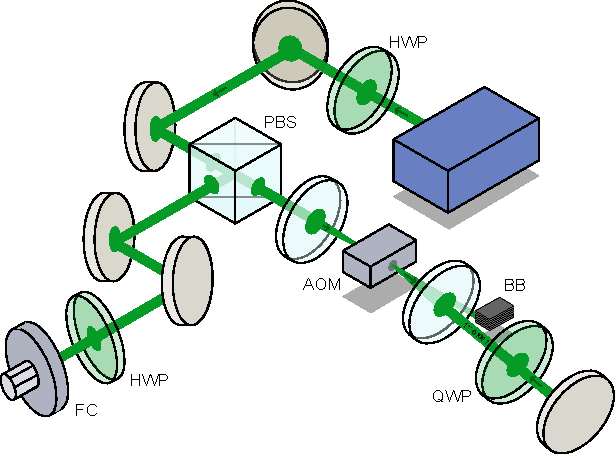
\includegraphics[width=0.95\textwidth]{../figures/excitation_aom.pdf}
    \caption{Simplified illustration of the excitation system, fiber coupled to the optical head. The labelled components are half-wave plate (HWP), quarter-wave plate (QWP), acousto optical modulator (AOM), polarizing beam splitter (PBS), beam block (BB), and fiber coupler (FC). The excitation begins at the laser module (blue), and passes twice through the AOM, and terminates at the fiber coupler.}
    \label{fig:exc_aom}
\end{figure}

The laser is an `Opus Gem' at \qty{532}{\nano\meter}. The linear polarized beam passes through the HWP, which is rotated for maximum transmission of the beam through the PBS. The beam is focused to a spot on the AOM, corresponding to the AOM crystal size specification. This ensures a rise/fall time of the modulated beam in specification, and a long lifetime of the AOM. The beams (0 and 1\textsuperscript{st} order) are collimated, and the 0 order beam is blocked. The 1\textsuperscript{st} order beam passes through a QWP twice, accumulating a rotation of \ang{180}, and passes back through the same path, through the AOM. The beam deflection acquired during the first pass is reversed during this second pass. This configuration is called the double-pass AOM configuration\cite{donleyDoublepassAcoustoopticModulator2005}. The beam is then reflected from the PBS due to the accumulated phase, and is coupled into a fiber. 

The advantage of using an AOM is a high extinction ratio and fast switching of the laser. This AOM driver also allows for easy control of the laser power with an analog voltage input, which allows for pulse sequences that require control of excitation power and relative control of power between different types of measurements.



\subsection*{Optical head}

\section{AFM modalities}

\section{SQM modalities}